\chapter{Ciclo di vita di un'azienda}
Ogni azienda attraversa fasi di crescita definite stadi del ciclo di vita\index{Organizzazione aziendale!Ciclo di vita}, che rappresentano la maturazione dell’organizzazione. 

\section{Stadi di sviluppo}
Gli stadi principali\index{Organizzazione aziendale!Ciclo di vita!stadi di sviluppo} sono quattro, come mostrato in Figura \ref{fig:ciclo-di-vita}:
\begin{enumerate}
    \item \textit{Stadio imprenditoriale:} In questo primo stadio, l’azienda si concentra sulla creazione del prodotto o servizio e sulla sopravvivenza nel mercato. La struttura organizzativa è informale e il controllo diretto è gestito dall’imprenditore. Col tempo, la crescita comporta un aumento del numero di dipendenti e di problematiche, portando a una "\textit{crisi di leadership}" in cui emerge la necessità di una direzione chiara.
    \item \textit{Stadio della collettività:} Superata la crisi di leadership, l’azienda sviluppa obiettivi e una direzione chiara. L’organizzazione inizia a formarsi con una prima gerarchia di autorità e divisione dei compiti, favorendo un ambiente in cui i dipendenti contribuiscono al successo aziendale. Tuttavia, questa struttura centrale conduce a una "\textit{crisi di delega}", poiché il management deve trovare nuovi metodi di controllo e coordinamento che non siano esclusivamente legati alla supervisione diretta.
    \item \textit{Stadio della formalizzazione:} In questo stadio si introducono regole e sistemi di controllo per migliorare la gestione. La comunicazione formale segue la linea gerarchica e si assumono figure specializzate. La direzione si concentra su strategia e pianificazione, mentre il management di medio livello gestisce le operazioni. L’organizzazione rischia però di soffocare sotto l’eccessiva burocrazia, portando a una "\textit{crisi da eccesso di burocrazia}".
    \item \textit{Stadio di elaborazione:} La crisi da eccesso di burocrazia si risolve sviluppando collaborazione e lavoro di squadra, riducendo la necessità di controlli formali. Si crea un ambiente favorevole alla gestione autonoma e alla decentralizzazione, evitando una crescita eccessiva della struttura formale. Col tempo (dai 10 ai 20 anni), l’organizzazione potrebbe necessitare di una "\textit{rivitalizzazione}", per rinnovarsi ed evitare il declino.
\end{enumerate}

\begin{figure}[ht]
    \centering
    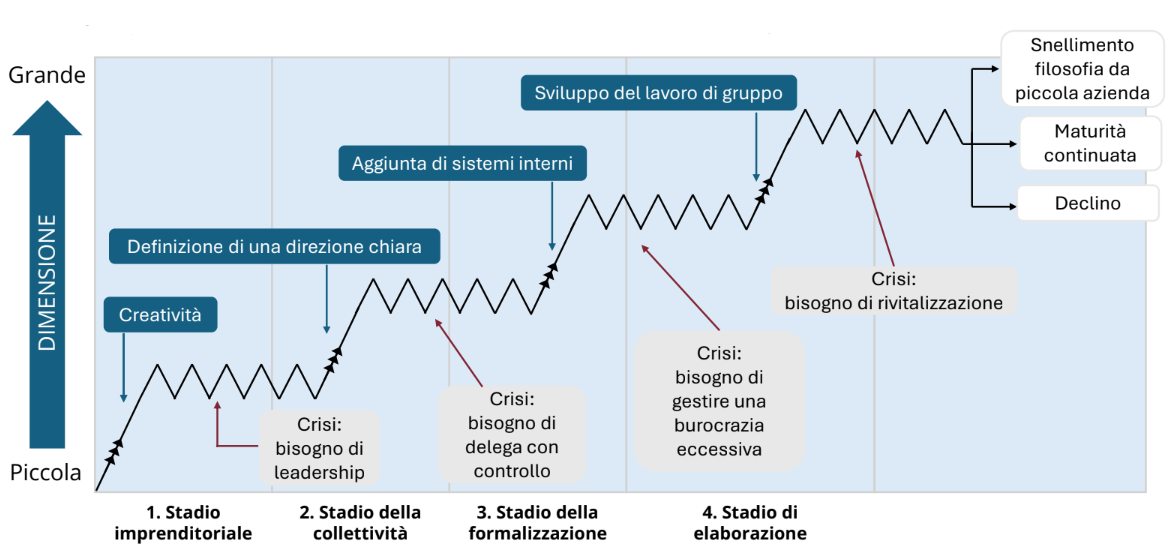
\includegraphics[width=0.8\linewidth]{images/ciclo-di-vita.PNG}
    \caption{Ciclo di vita di un'impresa}
    \label{fig:ciclo-di-vita}
\end{figure}

\begin{table}[ht]
\centering
\rowcolors{2}{lightblue}{lightgray}
\footnotesize
\begin{tabular}{|p{2cm}|p{2.5cm}|p{2.5cm}|p{3.5cm}|p{3.5cm}|}
\hline
\rowcolor{headerblue}
\textbf{\textcolor{white}{Caratteristiche}} & \textbf{\textcolor{white}{1. Imprenditoriale}} & \textbf{\textcolor{white}{2. Collettività}} & \textbf{\textcolor{white}{3. Formalizzazione}} & \textbf{\textcolor{white}{4. Elaborazione}} \\
\hline
\rowcolor{headerblue}
\textcolor{white}{Burocrazia} & \textcolor{white}{Non burocratica} & \textcolor{white}{Pre-burocratica} & \textcolor{white}{Burocratica} & \textcolor{white}{Molto burocratica}\\\hline
Struttura & Informale, dipendente da un singolo & Prevalentemente informale, qualche procedura & Procedure formali, divisione del lavoro, aggiunta di specializzazioni & Lavoro di gruppo all’interno di un contesto burocratico, approccio da piccola azienda\\\hline

Prodotti o servizi & Singolo prodotto o servizio & Prodotto o servizio principali con varianti & Linea di prodotti o servizi & Molteplici linee di prodotto o servizio\\\hline

Sistemi di ricompensa e di controllo & Personali, paternalistici & Personali, contributo al successo & Impersonali, sistemi formalizzati & Diffusi, personalizzati rispetto a prodotti e unità organizzative\\\hline

Innovazione & Da parte del proprietario-manager & Da parte di dipendenti e manager & Da parte di gruppi separati dedicati all’innovazione & Da parte di un centro di ricerca e sviluppo istituzionalizzato\\\hline

Obiettivi & Sopravvivenza & Crescita & Stabilità interna, espansione nel mercato & Reputazione, un’organizzazione completa\\\hline

Stile adottato dal top management & Individualistico, imprenditoriale & Carismatico, capace di fornire una direzione & Delega e controllo & Orientamento al gruppo, «attacco» alla burocrazia\\\hline
\end{tabular}
\caption{Caratteristiche degli stadi di sviluppo di un'azienda}
\end{table}

\section{Stadi del declino}
Il declino organizzativo è caratterizzato da cinque stadi\index{Organizzazione aziendale!Ciclo di vita!stadi di declino}, che se non gestiti correttamente possono portare alla dissoluzione dell’azienda, come mostato nella Figura \ref{fig:stati-del-declino}:
\begin{enumerate}
    \item \textit{Stadio della cecità:} In questa fase, cambiamenti interni ed esterni minacciano l’azienda (es. personale in eccesso, procedure troppo farraginose, mancanza di allineamento con i clienti, ecc.), ma il top management potrebbe non notare i segnali. Per prevenire questo stadio, è essenziale avere sistemi di monitoraggio che evidenzino le problematiche.
    \item \textit{Stadio dell’inattività:} Nonostante i segni di declino, il management ignora la realtà, convincendo sé stessi e gli altri che tutto vada bene. Riconoscere il problema in tempo e allinearsi con il contesto esterno sono azioni necessarie.
    \item \textit{Stadio dell’errore:} A questo punto i problemi sono ormai evidenti, e se l’azienda non reagisce con misure adeguate, rischia di fallire. Solitamente, si intraprendono azioni drastiche come la riduzione dei costi o il taglio del personale. Il top management deve ridurre l’incertezza dei dipendenti e degli altri stakeholder chiarendo i valori e fornendo informazioni.
    \item \textit{Stadio della crisi:} In questa fase l’organizzazione si trova in uno stato di caos, e l’unica soluzione consiste in una radicale riorganizzazione, che può includere la sostituzione del management e cambiamenti drastici nella strategia e cultura aziendale.
    \item \textit{Stadio della dissoluzione:} Questo è il punto finale del declino, in cui l’organizzazione non può più essere salvata. È necessario chiudere l’attività in modo ordinato per limitare il danno ai dipendenti e alla reputazione.
\end{enumerate}

\begin{figure}[ht]
    \centering
    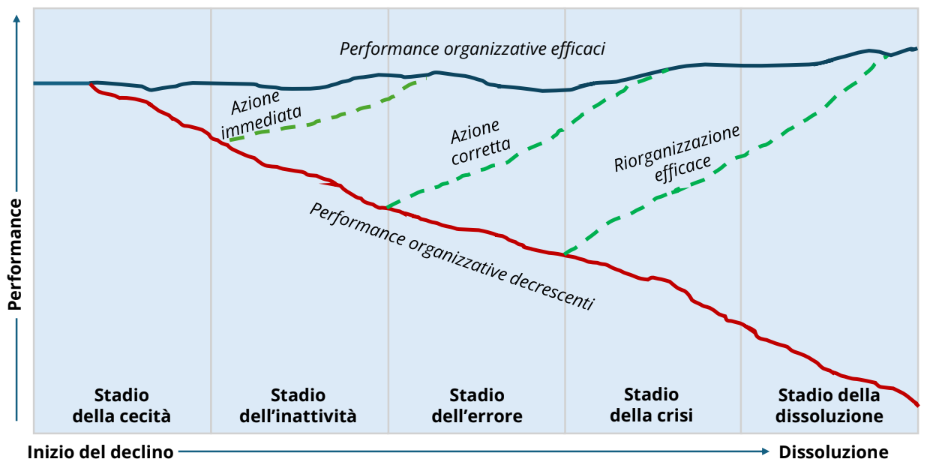
\includegraphics[width=0.7\linewidth]{images/stati-del-declino.PNG}
    \caption{Stati del declino}
    \label{fig:stati-del-declino}
\end{figure}